% !TEX encoding = Windows Latin 1
%paper prototype

\section{paper prototype}
\subsection{preparement}

After choosing our idea, we build a paper prototype for it. The prototype should help us to find a basic structure of our GUI before starting the real implementation. We sketched our views, a Web-Version and a android version. After many new tries we obtained our final version. We digitalized the results without any color.



\begin{figure}[!h]
        \begin{subfigure}[b]{0.5\textwidth}
                \centering
                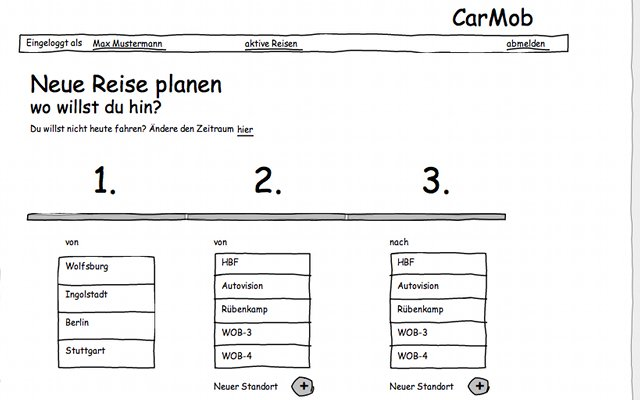
\includegraphics[width=\textwidth]{images/Web_1.jpg}
                \caption{searching a tour}
                \label{fig:web1}
        \end{subfigure}
        \begin{subfigure}[b]{0.5\textwidth}
                \centering
                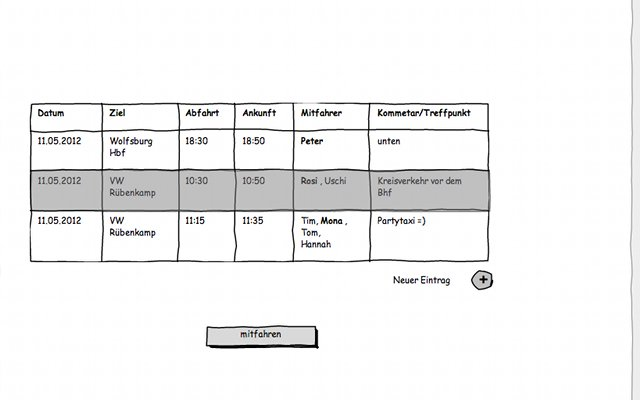
\includegraphics[width=\textwidth]{images/Web_2.jpg}
                \caption{choose a tour}
                \label{fig:web2}
        \end{subfigure}
                \caption{paper prototype: Web}
               \label{fig:web}
\end{figure}

\begin{figure}[!h]
        \begin{subfigure}[b]{0.3\textwidth}
                \centering
                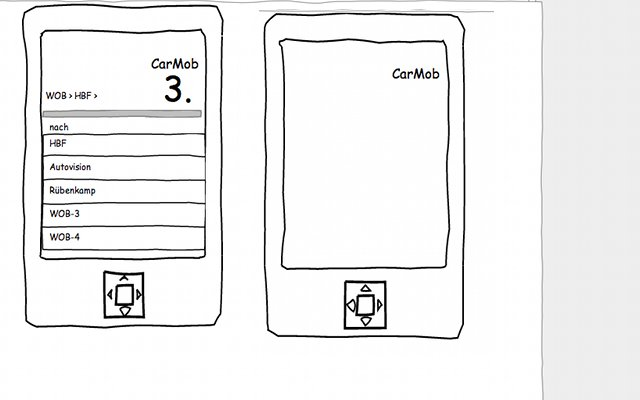
\includegraphics[width=\textwidth]{images/App_4.jpg}
                \caption{searching a tour}
                \label{fig:app1}
        \end{subfigure}
        \begin{subfigure}[b]{0.3\textwidth}
                \centering
                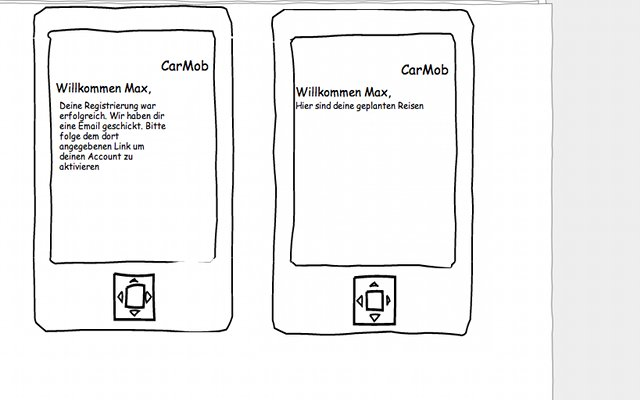
\includegraphics[width=\textwidth]{images/App_2.jpg}
                \caption{choose a tour}
                \label{fig:app2}
        \end{subfigure}
                \begin{subfigure}[b]{0.3\textwidth}
                \centering
                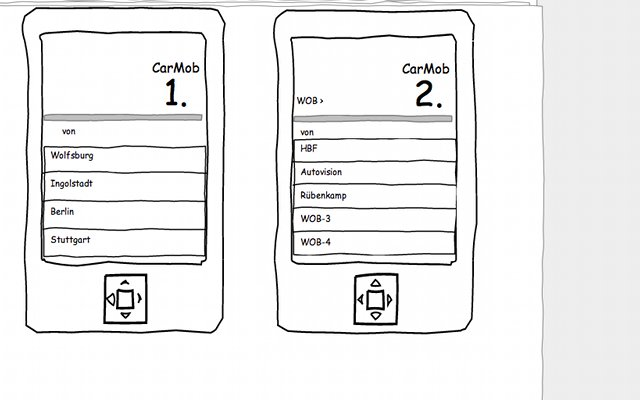
\includegraphics[width=\textwidth]{images/App_3.jpg}
                \caption{choose a tour}
                \label{fig:app3}
        \end{subfigure}
                \caption{paper prototype: App}
               \label{fig:web}
\end{figure}

\clearpage

\subsection{implementation}

During the tests it became clear, that nobody know why �active tours� means. For us it was a totally easy term. We found a lot of these misconceptions. But also semantic failures were offered. All things considered these test helped us a lot. And the best was they didn�t take much time.


\section{user stories}

We analyzed our requirements and split them in user stories with the style �the user wants to do x to do y�. We play card to calculate the time for each user story and its included tasks. We obtained the following user stories grouped by iterations

        \begin{figure}[!h]
                \centering
                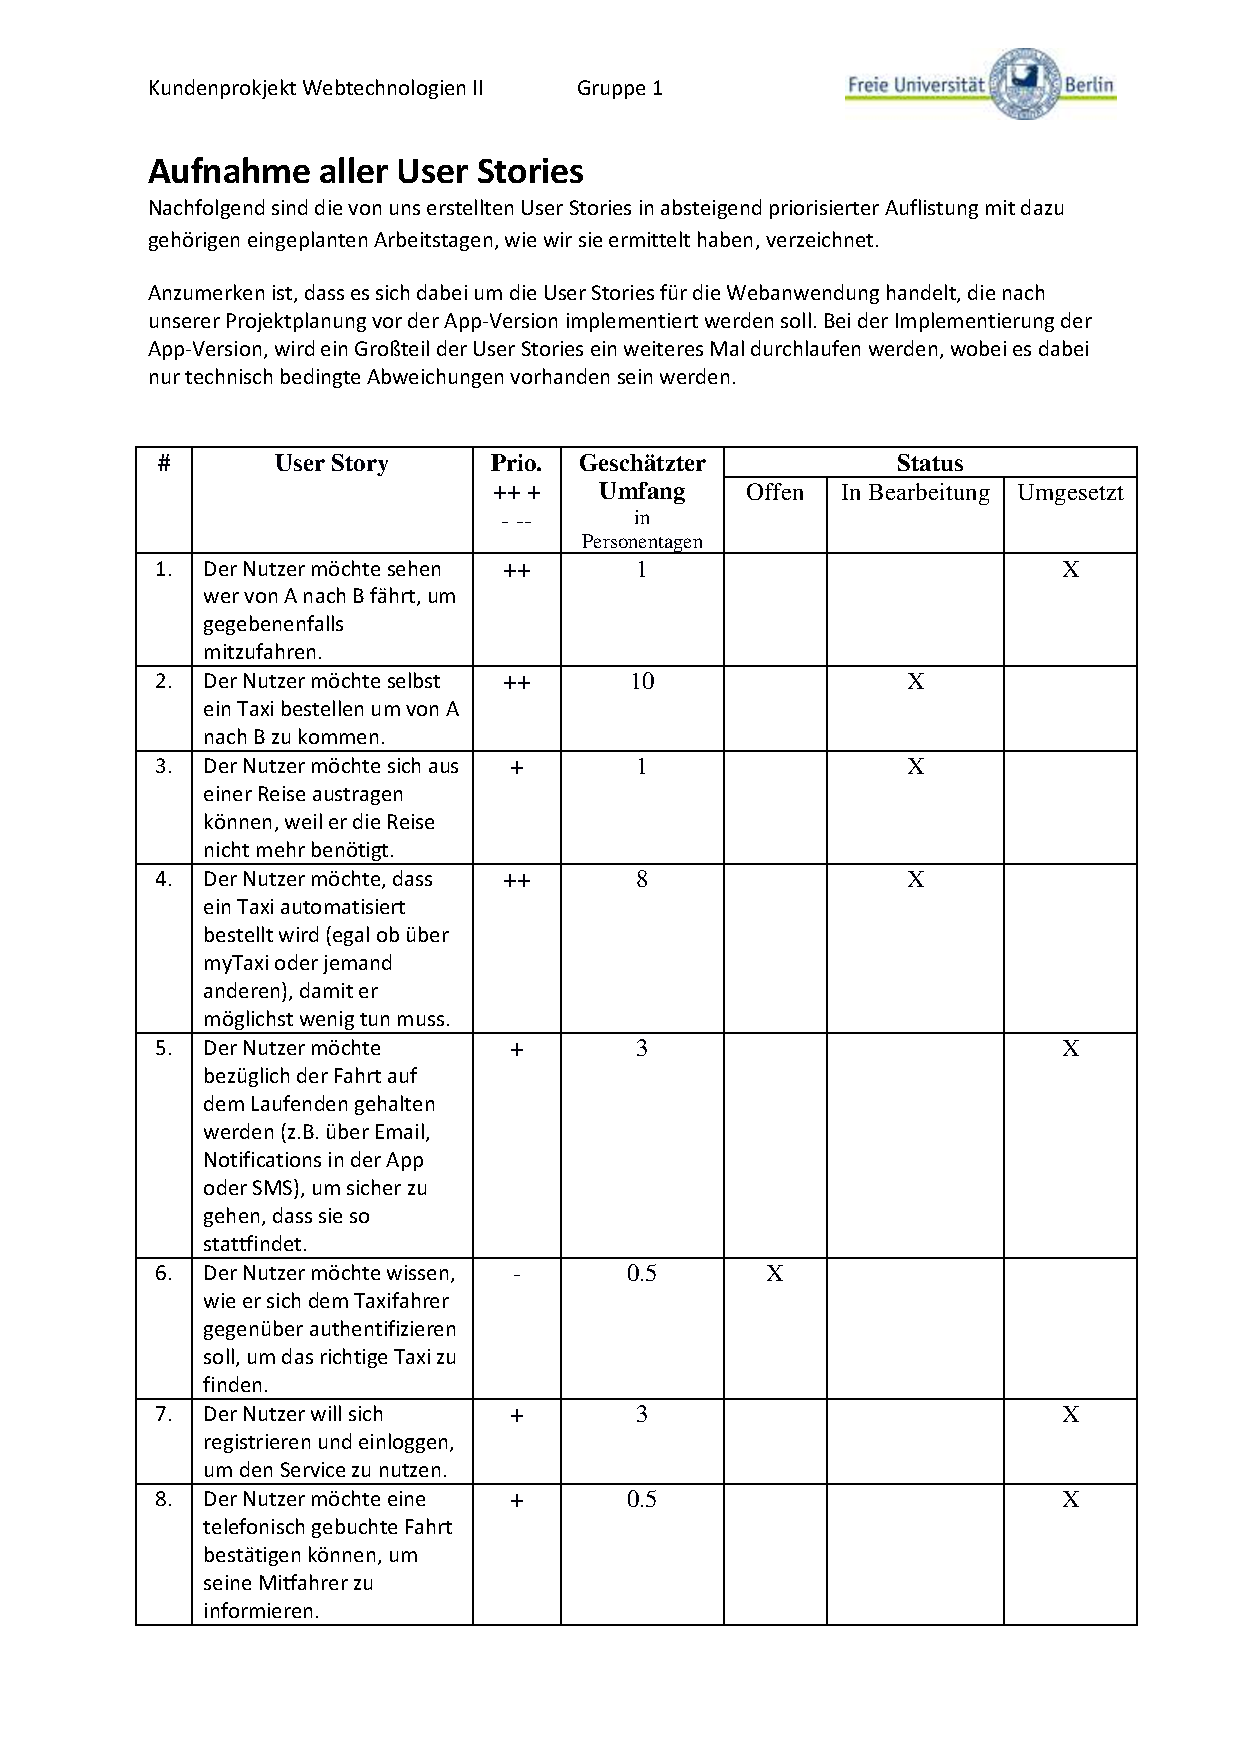
\includegraphics[width=\textwidth, page=1]{images/User_Stories.pdf}
                \caption{user stories sheet 1}
                \label{fig:user1}
        \end{figure}
        \qquad 
        
              \begin{figure}[!h]
                \centering
                \includegraphics[width=\textwidth, page=2]{images/User_Stories.pdf}
                \caption{user stories sheet 2}
                \label{fig:user2}
        \end{figure}
      \qquad 
                      \begin{figure}[!h]
                \centering
                \includegraphics[width=\textwidth, page=3]{images/User_Stories.pdf}
                \caption{user stories sheet 3}
                \label{fig:user3}
        \end{figure}
        \newpage
        
                      \begin{figure}[!h]
                \centering
                \includegraphics[width=\textwidth, page=4]{images/User_Stories.pdf}
                \caption{user stories sheet 4}
                \label{fig:user4}
        \end{figure}
        \newpage
                              \begin{figure}[!h]
                \centering
                \includegraphics[width=\textwidth, page=5]{images/User_Stories.pdf}
                \caption{user stories sheet 5}
                \label{fig:user5}
        \end{figure}
        
                                      \begin{figure}[!h]
                \centering
                \includegraphics[width=\textwidth, page=6]{images/User_Stories.pdf}
                \caption{user stories sheet 6}
                \label{fig:user6}
        \end{figure}
                                      \begin{figure}[!h]
                \centering
                \includegraphics[width=\textwidth, page=7]{images/User_Stories.pdf}
                \caption{user stories sheet 7}
                \label{fig:user7}
        \end{figure}
                                              \begin{figure}[!h]
                \centering
                \includegraphics[width=\textwidth, page=8]{images/User_Stories.pdf}
                \caption{user stories sheet 8}
                \label{fig:user8}
        \end{figure}
        
                                              \begin{figure}[!h]
                \centering
                \includegraphics[width=\textwidth, page=9]{images/User_Stories.pdf}
                \caption{user stories sheet 9}
                \label{fig:user9}
        \end{figure}
        
                                              \begin{figure}[!h]
                \centering
                \includegraphics[width=\textwidth, page=10]{images/User_Stories.pdf}
                \caption{user stories sheet 10}
                \label{fig:user10}
        \end{figure}
        
                                              \begin{figure}[!h]
                \centering
                \includegraphics[width=\textwidth, page=11]{images/User_Stories.pdf}
                \caption{user stories sheet 11}
                \label{fig:user11}
        \end{figure}
        
                                              \begin{figure}[!h]
                \centering
                \includegraphics[width=\textwidth, page=12]{images/User_Stories.pdf}
                \caption{user stories sheet 12}
                \label{fig:user12}
        \end{figure}
        
                                              \begin{figure}[!h]
                \centering
                \includegraphics[width=\textwidth, page=13]{images/User_Stories.pdf}
                \caption{user stories sheet 13}
                \label{fig:user13}
        \end{figure}
